\section{Testing and Results}\label{sec:testing_and_results}
TODO
\subsection{Delay Reduction of eBPF Forwarding}
When looking at the impact of eBPF-Forwarding on the delays of packets, we can see that
in the namespace environment the delay of a single packet is decreased by around 100\,µs
when compared to the userspace forwarding. This is shown in Figure~\ref{fig:delay-improvement} and 
consideres the simplest case of the userspace program where it only forwards directly to one connection
without the need for much additional computation. Given that the userspace can have arbitrary complex 
connection management this delay improvement can likely be even bigger in a more sophisticated userspace
setup.
\\
Another thing the figure shows is that the delay has a smaller variance due to the fact that the eBPF program
path is somewhat similar for each packet whereas, in contrast, the userspace path can have buffers, queues, 
or similar that lead to a higher difference in processing time between packets. 
This effect however might be less observable in a real world scenario due to the ubiquitous network jitter which 
was influencial in the used namespace environment.
\begin{figure}[htbp]
    \centering
    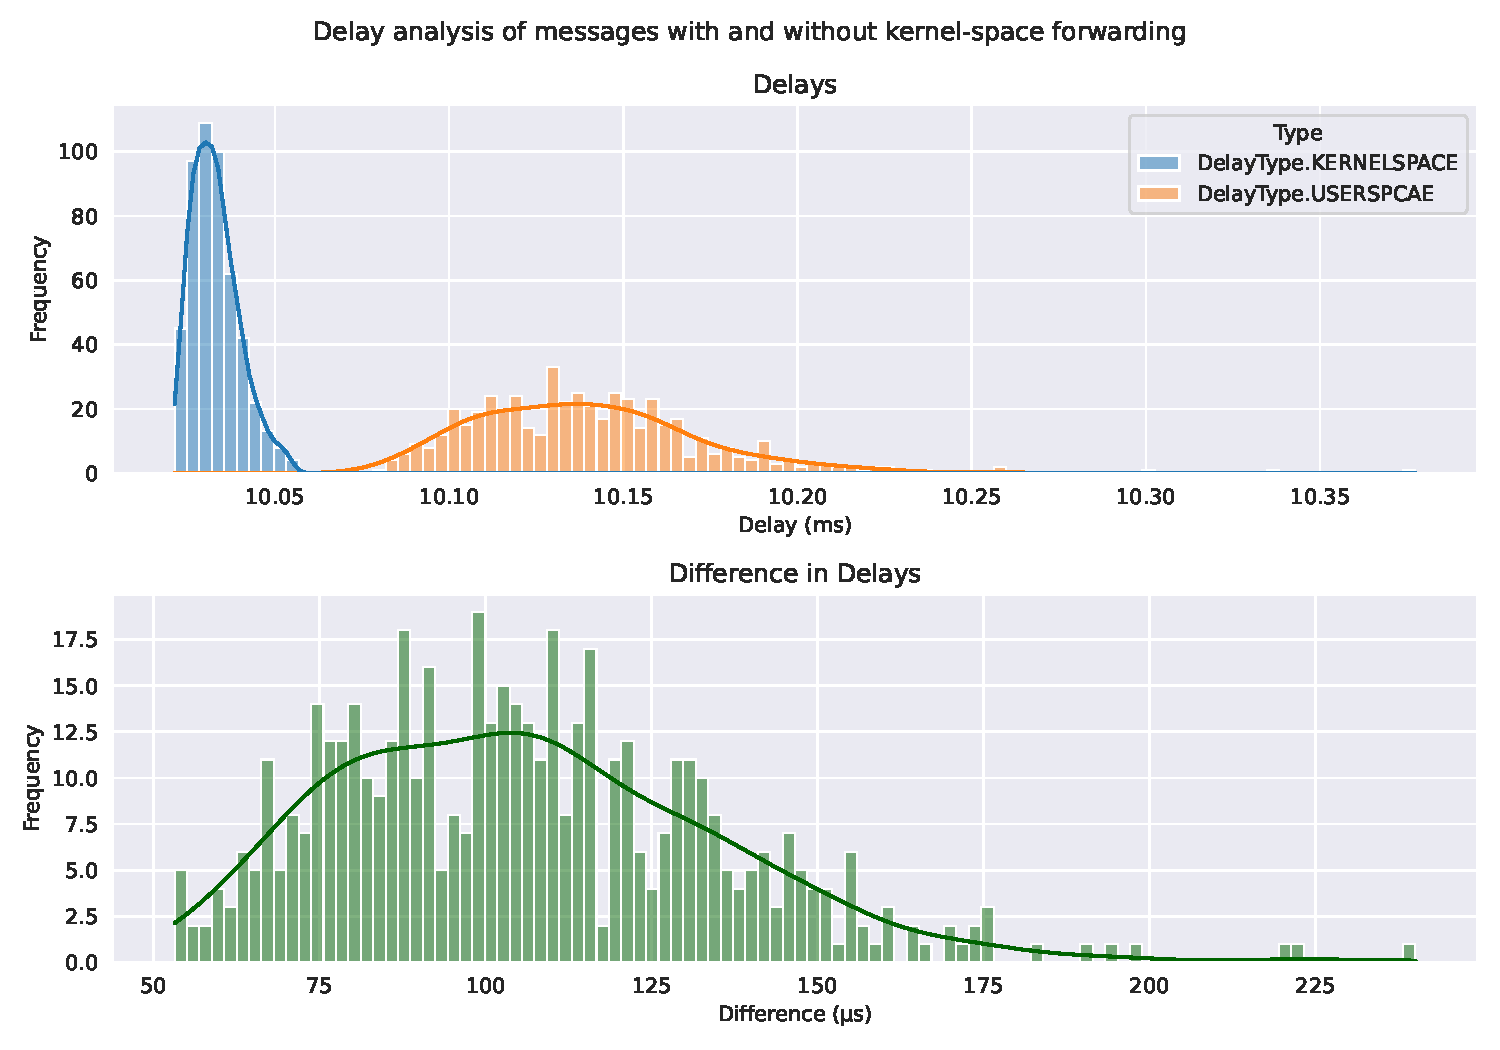
\includegraphics[width=\textwidth]{figures/04_testing_and_results/delays_small_packets_simple_userspace.pdf}
    \caption[Delay analysis of eBPF approach]{By avoiding userspace when processing the 1-RTT packets that contain the payload
    the delay of a single packet can be reduced. The longer-delay-operations are either handled
    directly in the eBPF program (e.g.~the case for deciding where to redirect a packet to) or 
    handled after the packet has already been sent out (e.g.~the case for registering a packet 
    such that the QUIC library knows about it).}\label{fig:delay-improvement}
\end{figure}
TODO

\subsection{CPU Utilization Comparison}
TODO

\begin{figure}[!htb]
    \begin{minipage}{0.48\textwidth}
        \centering
        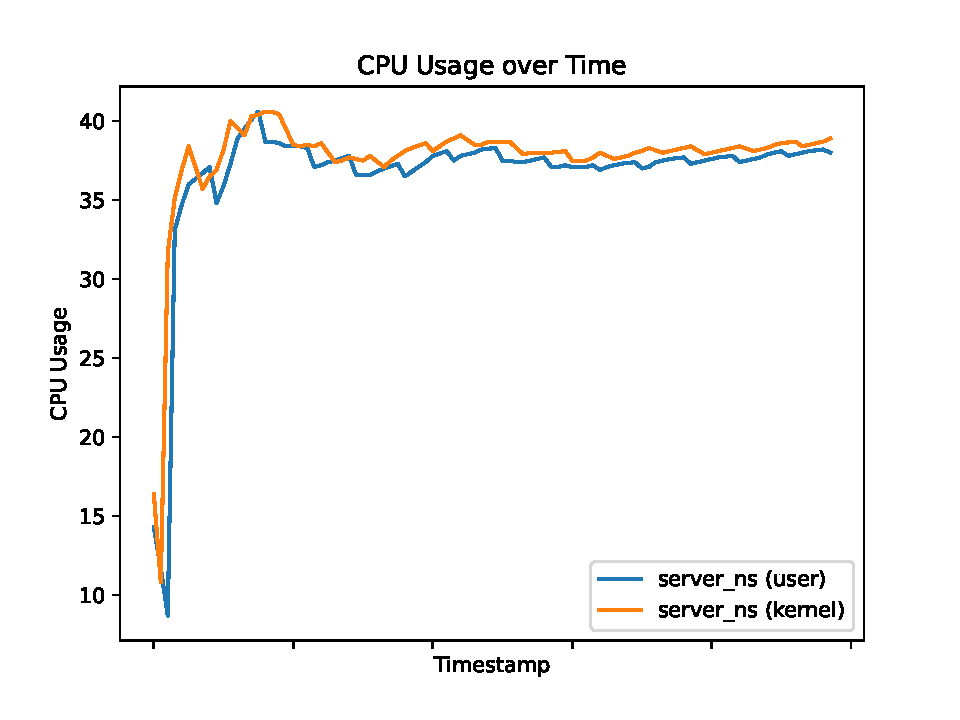
\includegraphics[width=1\linewidth]{figures/04_testing_and_results/cpu_usage_server_ns.pdf}
        \caption[Server CPU usage comparison]{Server namespace CPU usage comparison.}\label{fig:cpu-utilization-server}
    \end{minipage}\hfill
    \begin{minipage}{0.48\textwidth}
        \centering
        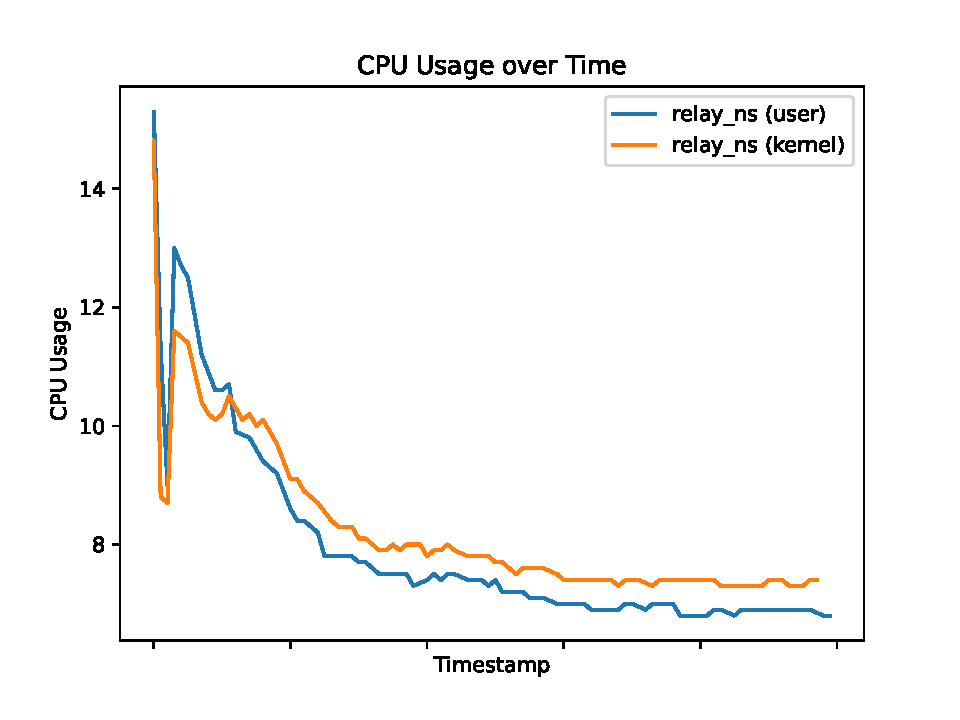
\includegraphics[width=1\linewidth]{figures/04_testing_and_results/cpu_usage_relay_ns.pdf}
        \caption[Relay CPU usage comparison]{Relay namespace CPU usage comparison.}\label{fig:cpu-utilization-relay}
    \end{minipage}\hfill
    \begin{minipage}{\textwidth}
        \centering
        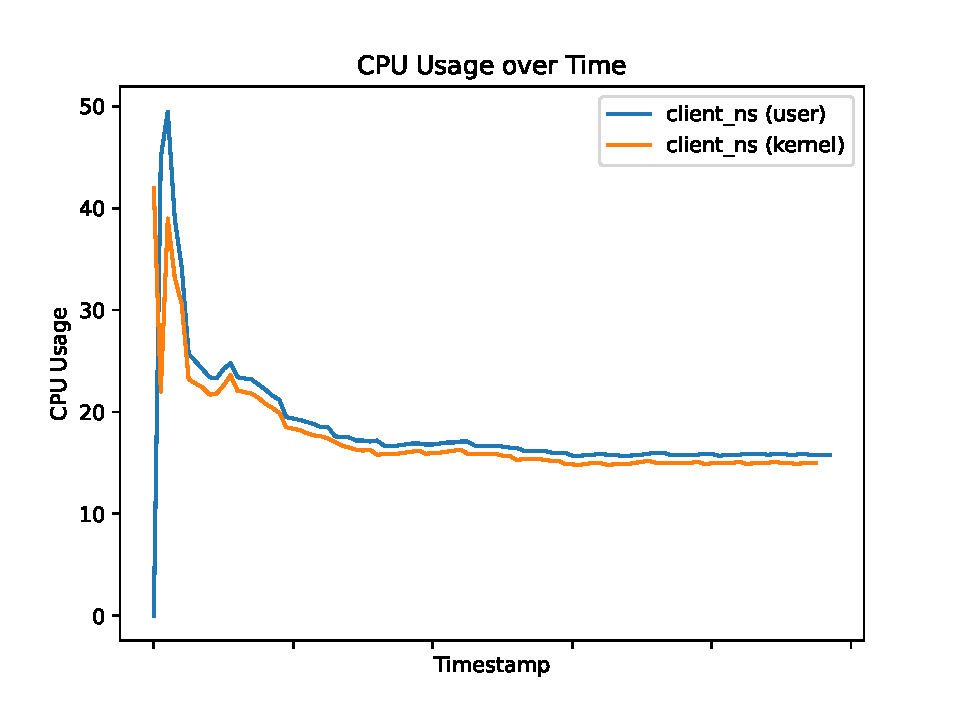
\includegraphics[width=0.48\textwidth]{figures/04_testing_and_results/cpu_usage_client_ns.pdf}
        \caption[Client CPU usage comparison]{Client namespace CPU usage comparison.}\label{fig:cpu-utilization-client}
    \end{minipage}
\end{figure}

\begin{table}
\caption{Table for CPU usage of relay Go processes}
\label{tab:cpu-usage-top}
\begin{tabular}{llllll}
\toprule
flat & flat\% & sum\% & cum & cum\% & cause \\
\midrule
440ms & 28.39\% & 28.39\% & 440ms & 28.39\% & runtime/internal/syscall.Syscall6 \\
140ms & 9.03\% & 37.42\% & 140ms & 9.03\% & runtime.futex \\
120ms & 7.74\% & 45.16\% & 120ms & 7.74\% & runtime.cgocall \\
40ms & 2.58\% & 47.74\% & 40ms & 2.58\% & runtime.write1 \\
30ms & 1.94\% & 49.68\% & 60ms & 3.87\% & runtime.checkTimers \\
30ms & 1.94\% & 51.61\% & 50ms & 3.23\% & runtime.mapaccess2 \\
20ms & 1.29\% & 52.90\% & 70ms & 4.52\% & .../cilium/ebpf/internal/unix.Syscall \\
20ms & 1.29\% & 54.19\% & 20ms & 1.29\% & net.IP.String \\
20ms & 1.29\% & 55.48\% & 20ms & 1.29\% & runtime.casgstatus \\
20ms & 1.29\% & 56.77\% & 20ms & 1.29\% & runtime.duffcopy \\
\bottomrule
\end{tabular}
\end{table}

% \begin{table}
\caption{Table for cumulative CPU usage of relay Go processes}
\label{tab:example}
\begin{tabular}{llllll}
\toprule
flat & flat\% & sum\% & cum & cum\% & cause \\
\midrule
0.44s & 28.39\% & 28.39\% & 0.44s & 28.39\% & runtime/internal/syscall.Syscall6 \\
0 & 0\% & 28.39\% & 0.43s & 27.74\% & runtime.mcall \\
0.01s & 0.65\% & 29.03\% & 0.42s & 27.10\% & runtime.schedule \\
0 & 0\% & 29.03\% & 0.41s & 26.45\% & runtime.park\_m \\
0 & 0\% & 29.03\% & 0.40s & 25.81\% & syscall.RawSyscall6 \\
0.01s & 0.65\% & 29.68\% & 0.32s & 20.65\% & runtime.findRunnable \\
0 & 0\% & 29.68\% & 0.28s & 18.06\% & .../quic-go-prio-packs.(*connection).run \\
0 & 0\% & 29.68\% & 0.28s & 18.06\% & syscall.Syscall \\
0 & 0\% & 29.68\% & 0.23s & 14.84\% & .../quic-go-prio-packs.(*Transport).listen \\
0 & 0\% & 29.68\% & 0.23s & 14.84\% & .../quic-go-prio-packs.(*connection).run.func2 \\
\bottomrule
\end{tabular}
\end{table}
 % TODO: this is kinda useless since it only shows the "wrapping" functions. Maybe remove?
TODO